\begin{figure}[p]
\centering
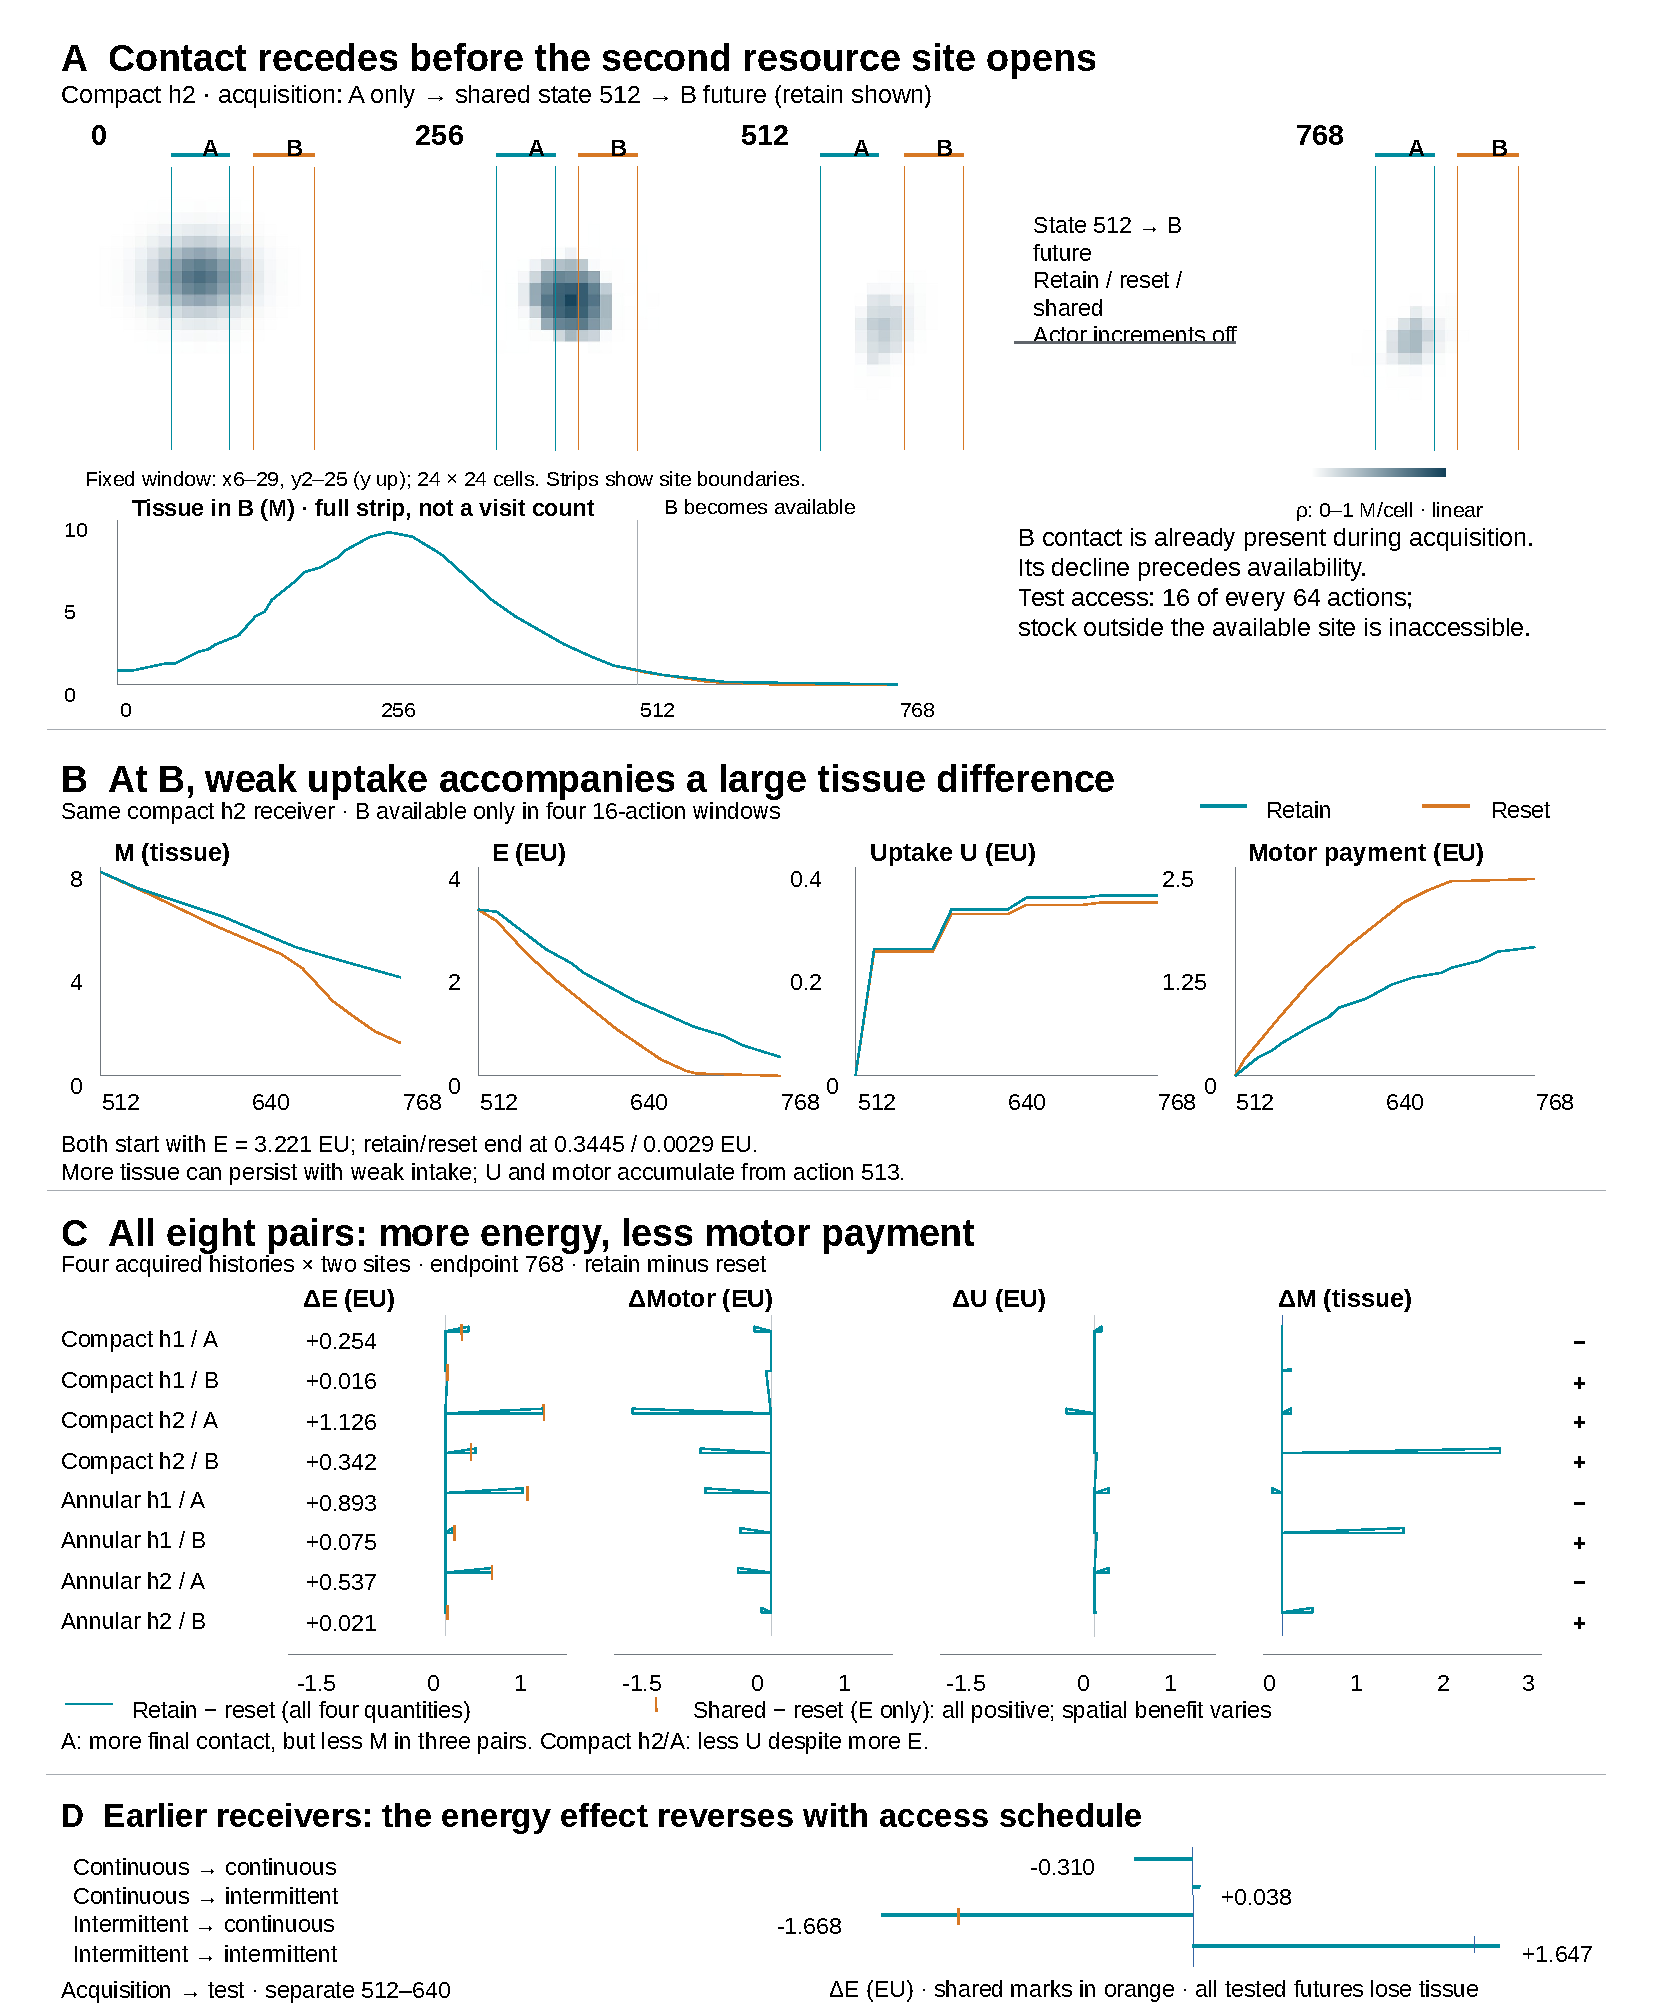
\includegraphics[width=0.94\linewidth]{figures/main/action_opportunity/action_opportunity.pdf}
\caption{\textbf{Retained actor state can preserve energy without restoring substantial uptake.}
\textbf{a,} Compact h2 body fields in one original-coordinate window (x6--29, y2--25; y upward), with common linear density scale. Lines locate resource strips, not stocks. Only A supplies during acquisition; B becomes available at 513. Full-strip B contact rises and then recedes before availability.
\textbf{b,} Absolute tissue, energy and cumulative uptake/motor payment from the same receiver at 512. Retaining more tissue accompanies weak uptake and reserve depletion.
\textbf{c,} All eight conditions from four histories and two future sites. Teal: retain minus reset; orange: shared minus reset for energy. The three EU quantities share a scale; tissue has its own scale. Higher A contact does not ensure more total tissue or uptake.
\textbf{d,} A separate earlier batch crosses two compact acquisition histories with two test schedules (512--640), giving opposite energy signs under continuous and intermittent access; orange marks add the one-receiver shared diagnostic. Actor increments are disabled throughout these tests. Initial mean probability matching does not match actions or payments. These conditional retained-state effects do not establish sustained adaptation.}
\label{fig:action-opportunity}
\end{figure}
